%File: model.tex
%Date: Fri Jan 03 21:06:49 2014 +0800
%Author: Yuxin Wu <ppwwyyxxc@gmail.com>

\subsection{GMM}
\textbf{Gaussian Mixture Model} is commonly used in acoustic learning task such as speech/speaker recognition,
since it describes the varied distribution of all the feature vector.\cite{GMM}
GMM assumes that the probability of a feature vector $x$ belonging to the model is the following:
\begin{equation}
p(x | w_i, \mu_i, \Sigma_i) = \sum_{i=1}^{K}{w_i \mathcal{N}(x | \mathbf{\mu}_i, \Sigma_i)}
\label{eqn:gmm}
\end{equation}

where
\[\mathcal{N}(x | \mathbf{\mu}_i, \Sigma_i) = \dfrac{1}{(2\pi)^{\frac{d}{2}}\sqrt{|\Sigma_i|}}
\exp \left({-\dfrac{1}{2}(x-\mu_i)^T\Sigma_i^{-1}(x-\mu_i)}\right)\]
subject to
\[\sum_{i=1}^{K} w_i = 1\]

  Therefore, GMM is merely a weighted combination of multivariate Gaussian distribution which
  assumes feature vectors are independent.
  (Actually we use diagonal covariances since the dimensions of the feature vector is independent to each other).
  GMM can describe the distribution of feature vector with several clusters, as shown in \figref{gmm-fig}
\begin{figure}[H]
  \centering
  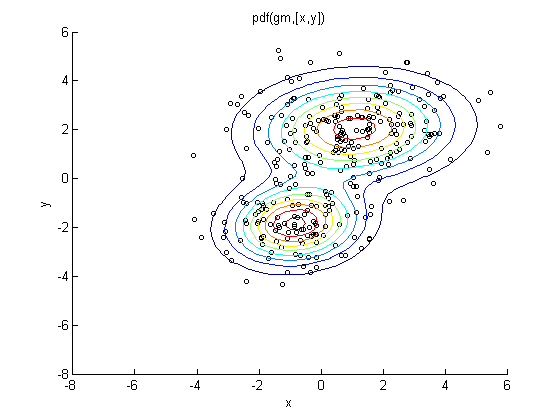
\includegraphics[width=0.8\textwidth]{img/gmm.png}
  \caption{A Two-Dimensional GMM with Two Components\label{fig:gmm-fig}}
\end{figure}

The training of GMM is the process to find the best parameters for $ \mu_i, \Sigma_i, w_i$,
so that the model fits all the training data with maximized likelihood.
More specifically, Expectation-Maximization(EM)
Algorithm\cite{bilmes1998gentle} is used to maximize the likelihood.
The two steps of one iteration of the algorithm in GMM training case here are
\begin{itemize}
	\item \textbf{E-Step} For each data point(feature vector), estimate the probatility that
		each Gaussian generated it\footnote{Actually, for an arbitrary point in
			space, its measure is zero, therefore its ``probability'' is
			actually zero. Therefore, here by ``probability of $x$'' we mean
			``the value of probability distribution function at $x$'' }.
			This is done by direct computation using \eqnref{gmm}.
	\item \textbf{M-Step} Modify the parameters of GMM such that maximize the
		likelihood of data. Here, hidden variable $z_{ij}$ is introduced
		to indicate where $i$-th data point is generate by Gaussian $j$.
		It can be shown that, instead of maximizing the
		likelihood of data, we can maximize the expectation of log likehood
		of data with respect to $Z$.

		let $\theta = \{w, \theta, \Sigma\}$, the log likehood function is
		\[Q(\theta', \theta) = \mathbb{E}_{Z} [\log p(X, Z) | \theta]\]
		where $\theta$ is current parameters, and $\theta'$ is the parameters
		we are to estimate. Incorporating the constraint $\sum_{i=1}^{K} w_i = 1$ using
		Lagrange multiplier gives
		\[J(\theta', \theta) = Q(\theta', \theta) - \lambda\left(\sum_{i=1}^{K} w_i - 1 \right)\]
		Set derivatives to zero, we can get the update equation
		\[Pr(i| x_j) = \dfrac{w_i \mathcal{N}(x_j | \mu_i', \Sigma_i')}{
			\sum_{k=1}^{K} w_k \mathcal{N}(x_j | \mu_k' \Sigma_k')}\]
		\[n_i = \sum_{j=1}^N Pr(i| x_j)\]
		\[\mu_i = \dfrac{1}{n_i} \sum_{t=1}^{T} Pr(i |x_j) x_j\]
		\[\Sigma_i = \left(\dfrac{1}{n_i} \sum_{t=1}^{T} Pr(i |x_j) diag(x_j x_j^T)\right) -
		diag(\mu_i' \mu_i'^T)\]
		\[w_i = \dfrac{n_i}{N}\]

\end{itemize}



After training, the model can give the score of fitness for every input feature vector,
measuring the probability that the vector belongs to this model.

Therefore, in the task of speaker recognition, we can train a GMM for every speaker.
Then for a input signal, we extract lists of feature vectors for it, and calculate the
overall likelihood that the vectors belong to each model.
The speaker whose model fits the input best will be choosen as the answer.

Moreover, an enhancement have been done to the original GMM method.
The training of GMM first requires a random initialization of the means of
all the components. However, we can first use K-Means algorithm\cite{kmeans} to perform a clustering
to all the vectors, then use the clustered centers to initialize the training of GMM.
This enhancement can speed up the training, also gives a better training result.

On the calculation of K-Means, an algorithm call K-MeansII\cite{bahmani2012scalable},
which is an improved version of K-Means++\cite{arthur2007k} can be used for better accuracy.

%\begin{itemize}
  %\item Performance: \\ We investigate the effect of initialization of GMM during
    %training. We implemented GMM with
    %K-meansII\cite{bahmani2012scalable}, which is an improved
    %version of K-means++\cite{arthur2007k} to initialize the
    %mean vector of GMM. Results shows improvements compared
    %to GMM provided by \textbf{scikit-learn\cite{scikit-learn}}.
  %\item Efficiency:
    %\begin{itemize}
      %\item We provide a parallel version of GMM, especially
        %optimized to train large Universal Background Model(UBM).
      %\item We further improve efficiency by utilizing
        %SSE instruction in computing exponential function
        %using polynomial approximation. This can speed up
        %the training procedure by a factor of two.
    %\end{itemize}
%\end{itemize}

\subsection{UBM}

\textbf{Universal Background Model} is a GMM trained on giant number of speakers.
It therefore describes common acoustic features of human voices.\cite{UBM}

As we are providing continuous speech close-set diarization function in
GUI, we adopt \textbf{Universal Background Model} as imposter model using equation
given in \cite{reynolds2000speaker}
and use likelihood ratio test to make reject decisions as proposed in\cite{reynolds2000speaker}.

Further more, by hints mentioned in paper, we only update mean vectors.

When using conversation mode in GUI (will be present later),
GMM model of each user is adapted from a pre-trained UBM
using method described in \cite{reynolds2000speaker}.

\subsection{CRBM}

\textbf{Restricted Boltzmann Machine} is generative stochastic
two-layer neural network that can learn a probability distribution
over its set of binary inputs\cite{rbm_wiki}.  \textbf{Continuous
restricted Boltzmann Machine(CRBM)}\cite{chen2003continuous} extends
its ability to real-valued inputs.  RBM has a ability to, given an
input(visible layer), reconstruct a hidden layer that is similar
to the input.  The neurons
in hidden layer controls the model complexity and the performance of
the network. The Gibbs sampling of hidden layer can be seen as a
representation of the original data. Therefore RBMs can be used
as an auto feature-extractor.
\figref{crbm} illustrate original MFCC data and the
sampled output of reconstructed data from CRBM.

Both RBM and CRBM can be trained using Contrastive Divergence learning,
with subtle difference in update equation.

As details about CRBM are too verbose to be covered here, for interested,
we recommend reading original papers.

Previous works using neural network largely focused on speech
recognition, such as \cite{deep},\cite{mohamed2011deep}.

\begin{figure}[H]
  \begin{minipage}{0.48\linewidth}
    \centering
    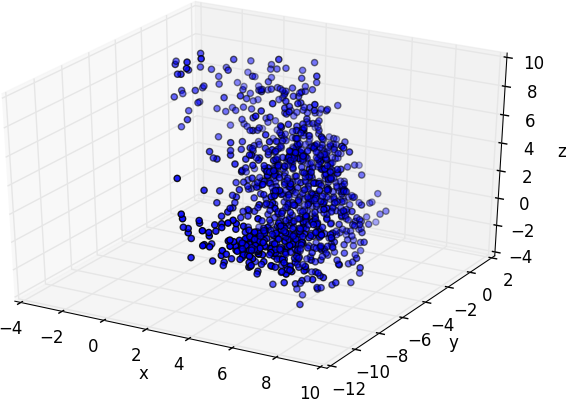
\includegraphics[width=\linewidth]{img/rbm-original.png}
    \caption*{The first three dimension of a woman's MFCC feature}
  \end{minipage}
  \hfill
  \begin{minipage}{0.48\linewidth}
    \centering
    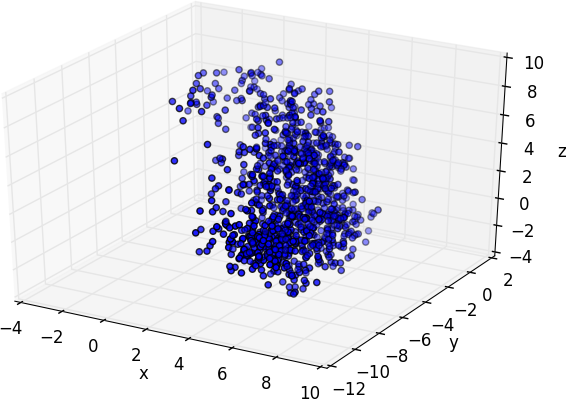
\includegraphics[width=\linewidth]{img/rbm-reconstruct.png}
    \caption*{The first three dimension of the same woman's MFCC feature
      recontructed by a CRBM with 50-neuron hidden layer. We can
      see that, the density of these two distributions are alike}
  \end{minipage}
  \caption{\label{fig:crbm}}
\end{figure}

To use CRBM as a substitution of GMM, rather than
an feature extractor, we train a CRBM per speaker,
and estimate reconstruction error without sampling (which is stable).
The person whose corresponding CRBM has lowest reconstruction error is chosen as

recognition result.

\subsection{JFA}

\textbf{Factor Analysis} is a typical method which behave
very well in classification problems, due to its ability to
account for different types of variability in training data.
Within all the factor analysis methods,
Joint Factor Analysis (JFA)\cite{jfa2,jfa-se} was proved to outperform other method
in the task of Speaker Recognition.

JFA models the user by ``supervector'' , i.e. a $C\times F $ dimension vector, where $C$ is
the number of components in the Universal Background Model, trained by GMM on all the training data,
and $ F$ is the dimension of the acoustic feature vector. The supervector of an utterance is obtained by concatenate
all the $C $ means vectors in the trained GMM model. The basic assumption of JFA on describing a supervector is:

\[ \vec{M} = \vec{ m } + vy + dz + ux, \]

where $m$ is a supervector usually selected to be the one trained from UBM, $v$ is a $ CF \times R_s$ dimension matrix,
$ u$ is a $ CF \times R_c$ dimension matrix, and $d$ is a diagonal matrix.
This four variables are considered independent of all kinds of variabilities and remain constant after training, and
$x, y, z $ are matrixes computed for each utterance sample.
In this formulation, $ m + vy + dz$ is commonly believed to account for the ``Inter-Speaker Variability'', and $ux $ accounts
for the ``Inter-Channel Variability''.
The parameter $ R_s $ and $ R_c$, also referred to as ``Speaker Rank'' and ``Channel Rank'', are two emprical constant selected as first.
The training of JFA is to calculate the best $ u, v, d$ to fit all the training data.

